\chapter{Verteilungssicht}
\label{ch:Verteilungssicht}
In der Verteilungssicht werden wir uns nun mit der Infrastruktur unserer Architektur befassen. Sie veranschaulicht den technischen Ablauf in unserem System und spiegelt dies in Form der gewählten Hardwarekomponenten sowie des in Abbildung \ref{fig:verteilung} veranschaulichten UML-Deployment Diagram wieder.

\begin{figure}[h]
	\centering
	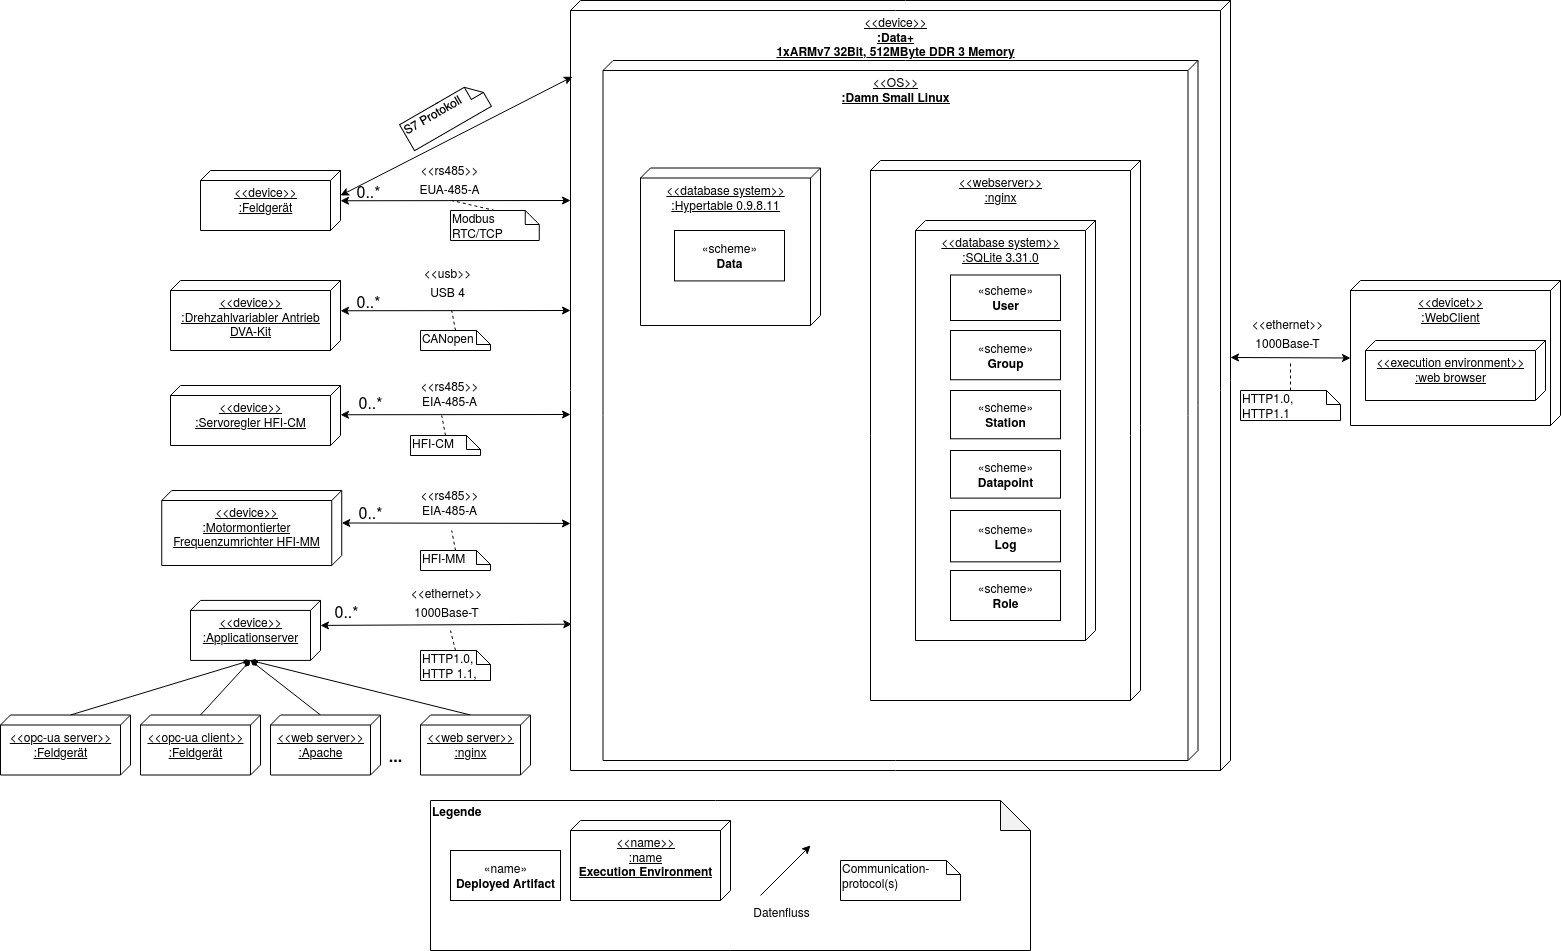
\includegraphics[width=1.1\textwidth]{Graphics/verteiler.png}
	\caption{Verteilungssicht der Anwendung}
	\label{fig:verteilung}
\end{figure}

Wie in der Abbildung zu sehen ist, besitzt das Device zwei Datenbanksysteme unterschiedlichen Typs. Zum einen eine relationale SQLite-Datenbank zum erfassen und verwalten von Konfigurationen, Systemzustand und Benutzerverwaltung, als auch eine Wide-Column-Store Hypertable-Datenbank zum speichern von eingehenden Betriebsdaten.
Die Funktionalität einer Weboberfläche wird mittels ngnix-Webserver, der auf die Daten der relationalen Datenbank zugreift bereitgestellt. Jedes der externen Geräte wird an einen der möglichen physikalischen Ports angebunden. Da hier unter anderem Bussysteme verwendet werden, muss davon ausgegangen werden, das mehrere Geräte auf einem Physikalischen Port angeschlossen sein können. Dabei veranschaulicht die Abbildung \ref{fig:verteilung} nicht die physikalisch möglichen Anschlüsse, sondern die logischen. An das System können verschiedene Bussysteme und Netze gleichzeitig angeschlossen werden. Die Anzahl der mit dem Device verbundenen Geräte wird dabei lediglich durch die Bus-/Netzwerkspezifische Maximalgröße und die Anzahl physikalischer Ports beschränkt. Allgemein unterstützt das System die Kommunikation mit den Bussystemen Modbus RTC/TCP, CAN/CANopen, HFI-CM, HFI-MM und Protokollen S7, HTTP1.0 und HTTP1.1.  